\chapter{Strukturaufklärung der Chl-Kataboliten mit ESI-MS}

\section{Identifizierte Chl-Kataboliten}

\subsection{Bo-DYCC}

\begin{figure}[!htbp]
  \centering
  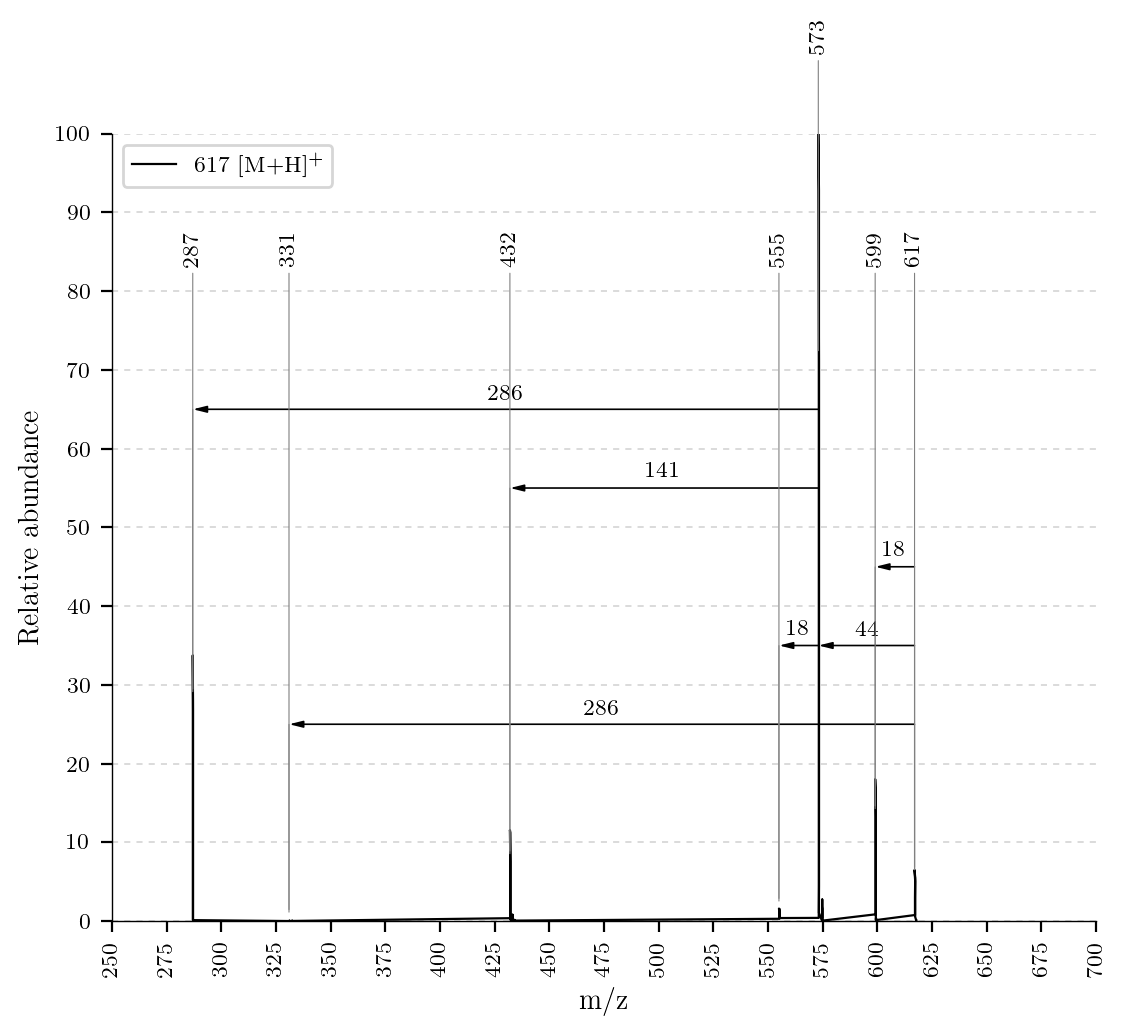
\includegraphics[width=\textwidth, height=0.7\textwidth]{figures/Kapitel7/Kataboliten/VWA_MS_617.png}
  \caption[LC-MS Chromatogramm vor der Reaktion, Quelle: Author]{\gls{lcms} Chromatogramm}
  \label{fig:LCMSChromatogramm}
\end{figure}

\begin{figure}[!htbp]
  \centering
  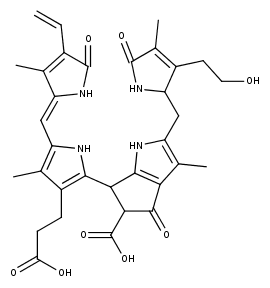
\includegraphics[scale=0.6]{figures/Kapitel7/Kataboliten/fragmentation_structures/VWA_Katabolit_617.png}
  \caption[LC-MS Chromatogramm vor der Reaktion, Quelle: Author]{\gls{lcms} Chromatogramm}
  \label{fig:LCMSChromatogramm}
\end{figure}

\begin{figure}[!htbp]
  \begin{subfigure}[b]{0.5\textwidth}
    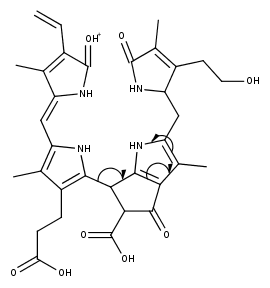
\includegraphics[width=\textwidth]{figures/Kapitel7/Kataboliten/fragmentation_structures/VWA_Katabolit_617_MH_RingD-RingC_331_electronMovement.png}
    \caption{}
    \label{fig:NCC2725}
  \end{subfigure}
  \hfill
  \begin{subfigure}[b]{0.5\textwidth}
    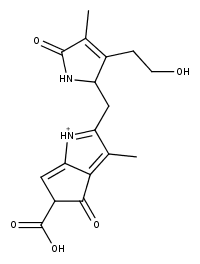
\includegraphics[width=\textwidth]{figures/Kapitel7/Kataboliten/fragmentation_structures/VWA_Katabolit_617-RingD-RingC_331.png}
    \caption{}
    \label{fig:DNCC2991}
  \end{subfigure}
  \caption[Online-UV/Vis Spektren mit der Charakteristik eines NCC bei 27.10min., eines DNCC bei 29.75min. sowie eines YCC bei 30.94min., Quelle: Autor]{Online-UV/Vis Spektren: (a) charakteristisch für einen \gls{NCC} - RT = 27.25min., (b) charakteristisch für einen \gls{DNCC} - RT = 29.91min., (c) charakteristisch für einen \gls{YCC} - RT = 30.94min.}
\end{figure}

\subsection{Bo-DNCC}

\begin{figure}[!htbp]
  \centering
  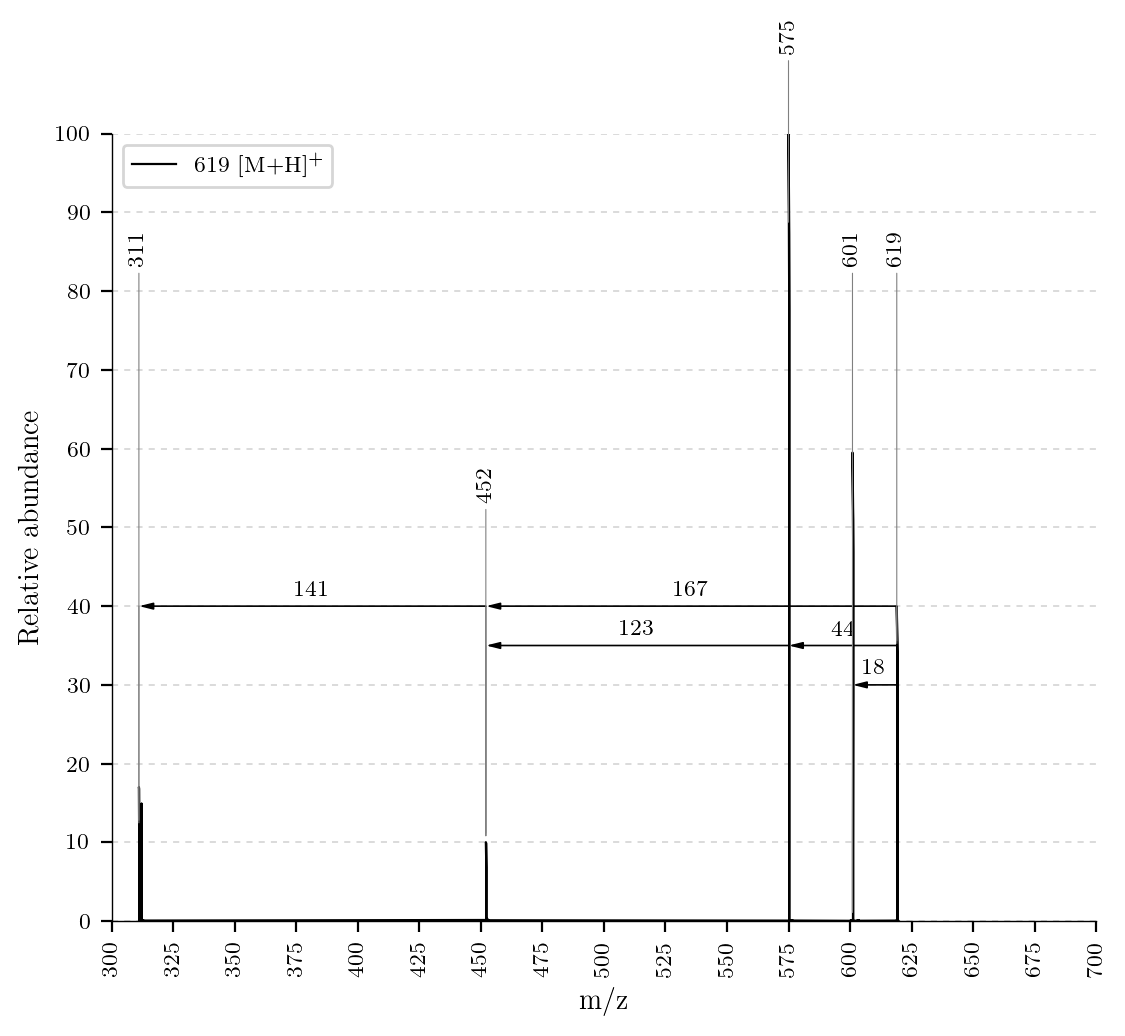
\includegraphics[width=\textwidth, height=0.7\textwidth]{figures/Kapitel7/Kataboliten/VWA_MS_619.png}
  \caption[LC-MS Chromatogramm vor der Reaktion, Quelle: Author]{\gls{lcms} Chromatogramm}
  \label{fig:LCMSChromatogramm}
\end{figure}

\begin{figure}[!htbp]
  \begin{subfigure}[b]{0.5\textwidth}
    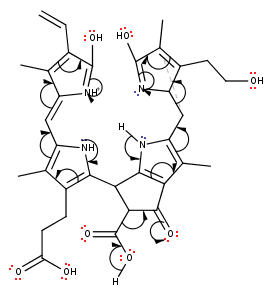
\includegraphics[width=\textwidth]{figures/Kapitel7/Kataboliten/fragmentation_structures/VWA_Katabolit_619_MH-CO2-RingA-RIngD_311_electronMovement.png}
    \caption{}
    \label{fig:NCC2725}
  \end{subfigure}
  \hfill
  \begin{subfigure}[b]{0.5\textwidth}
    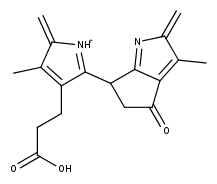
\includegraphics[width=\textwidth]{figures/Kapitel7/Kataboliten/fragmentation_structures/VWA_Katabolit_619-CO2-RingA-RingD_311.png}
    \caption{}
    \label{fig:DNCC2991}
  \end{subfigure}
  \caption[Online-UV/Vis Spektren mit der Charakteristik eines NCC bei 27.10min., eines DNCC bei 29.75min. sowie eines YCC bei 30.94min., Quelle: Autor]{Online-UV/Vis Spektren: (a) charakteristisch für einen \gls{NCC} - RT = 27.25min., (b) charakteristisch für einen \gls{DNCC} - RT = 29.91min., (c) charakteristisch für einen \gls{YCC} - RT = 30.94min.}
\end{figure}

\begin{figure}[!htbp]
  \begin{subfigure}[b]{0.5\textwidth}
    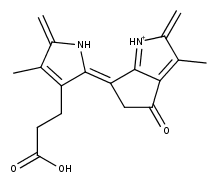
\includegraphics[width=\textwidth]{figures/Kapitel7/Kataboliten/fragmentation_structures/VWA_Katabolit_619-CO2-RingD-RingA_311_Mesomer1.png}
    \caption{}
    \label{fig:NCC2725}
  \end{subfigure}
  \hfill
  \begin{subfigure}[b]{0.5\textwidth}
    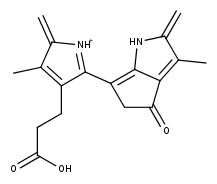
\includegraphics[width=\textwidth]{figures/Kapitel7/Kataboliten/fragmentation_structures/VWA_Katabolit_619-CO2-RingD-RingA_311_Mesomer2.png}
    \caption{}
    \label{fig:DNCC2991}
  \end{subfigure}
  \caption[Online-UV/Vis Spektren mit der Charakteristik eines NCC bei 27.10min., eines DNCC bei 29.75min. sowie eines YCC bei 30.94min., Quelle: Autor]{Online-UV/Vis Spektren: (a) charakteristisch für einen \gls{NCC} - RT = 27.25min., (b) charakteristisch für einen \gls{DNCC} - RT = 29.91min., (c) charakteristisch für einen \gls{YCC} - RT = 30.94min.}
\end{figure}

\subsection{Bo-YCC}

\begin{figure}[!htbp]
  \centering
  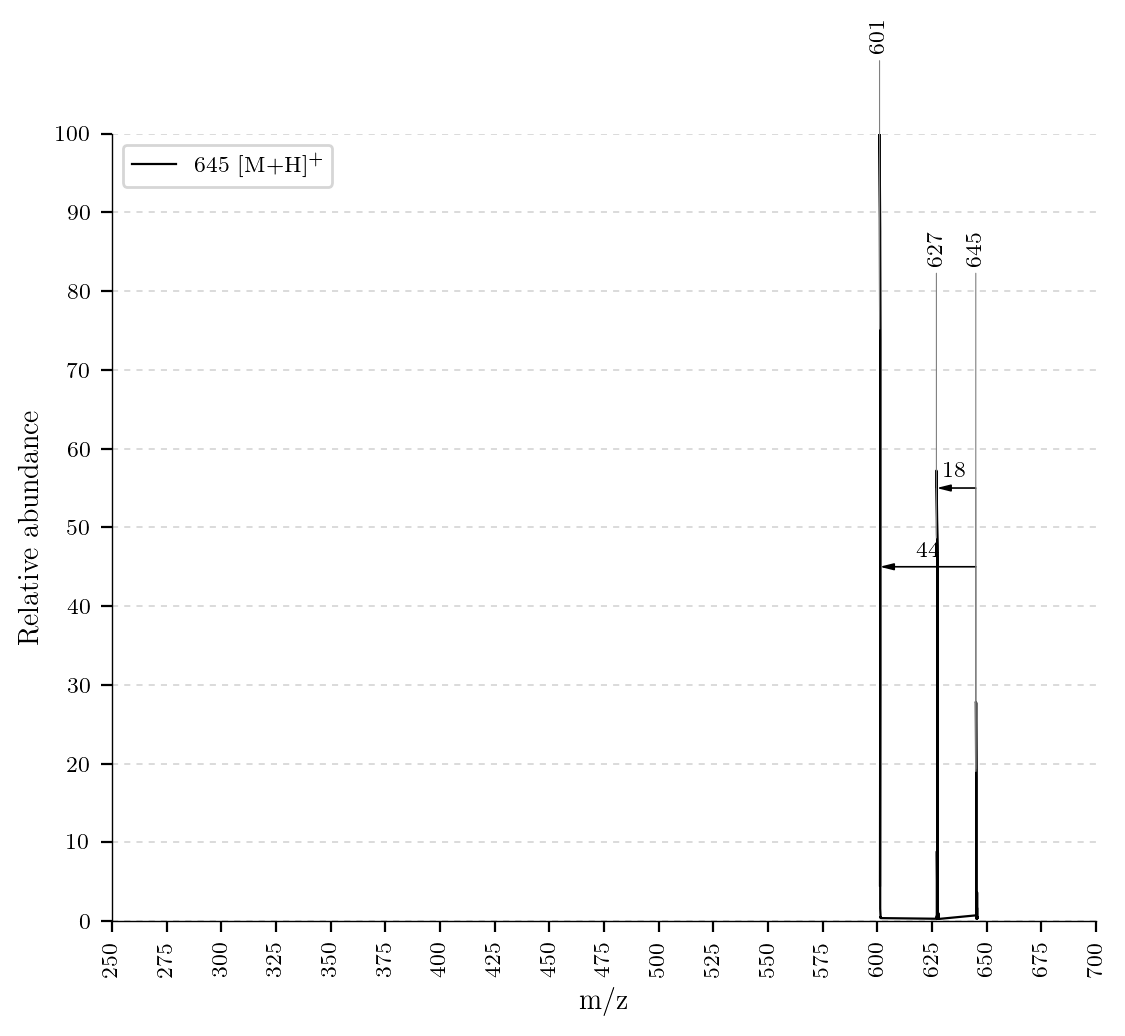
\includegraphics[width=\textwidth, height=0.7\textwidth]{figures/Kapitel7/Kataboliten/VWA_MS_645-1.png}
  \caption[LC-MS Chromatogramm vor der Reaktion, Quelle: Author]{\gls{lcms} Chromatogramm}
  \label{fig:LCMSChromatogramm}
\end{figure}

\begin{figure}[!htbp]
  \centering
  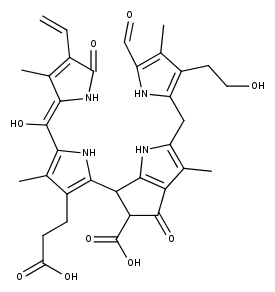
\includegraphics[scale=0.6]{figures/Kapitel7/Kataboliten/fragmentation_structures/VWA_Katabolit_645_vorReaktion.png}
  \caption[LC-MS Chromatogramm vor der Reaktion, Quelle: Author]{\gls{lcms} Chromatogramm}
  \label{fig:LCMSChromatogramm}
\end{figure}

\subsection{Bo-NCC-3}

\begin{figure}[!htbp]
  \centering
  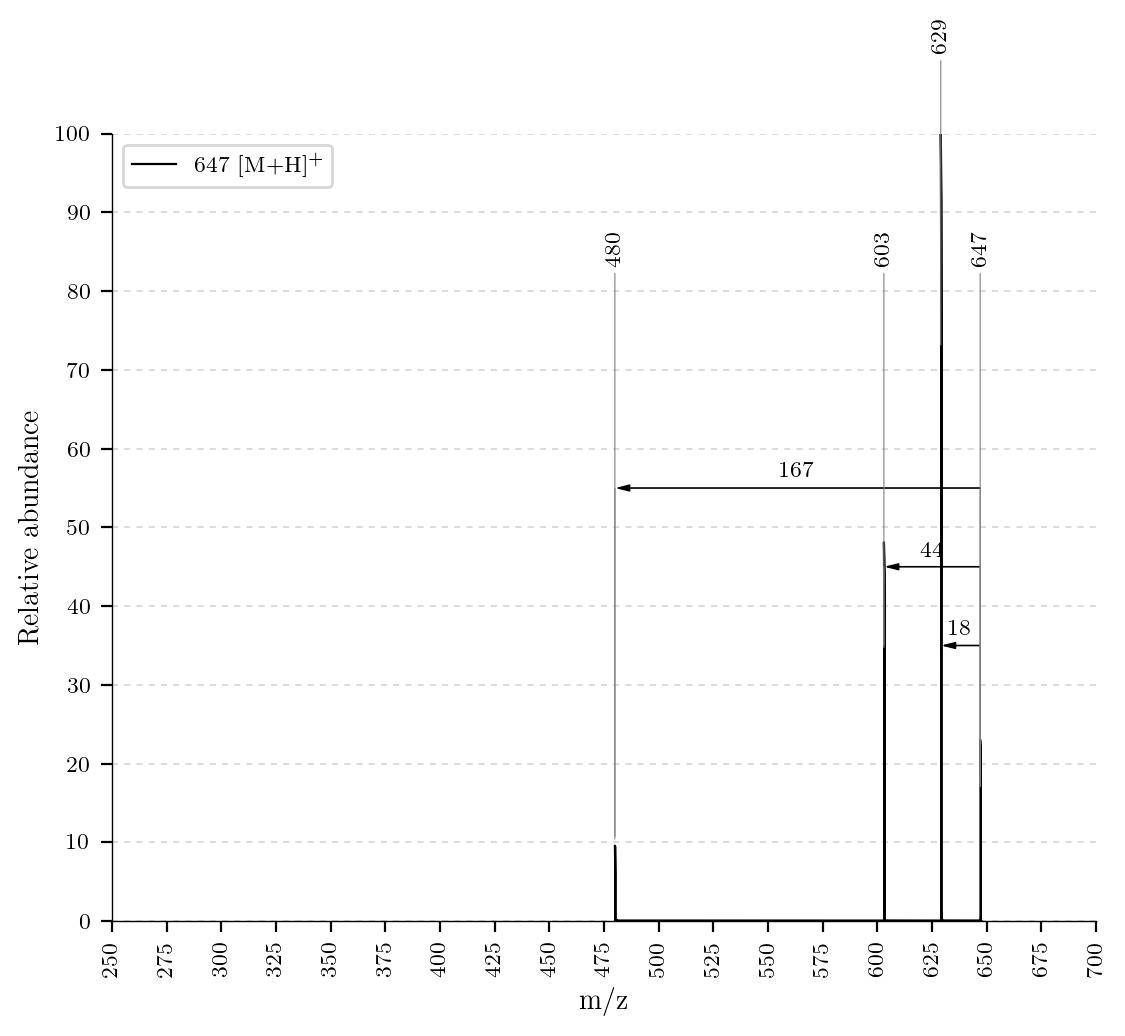
\includegraphics[width=\textwidth, height=0.7\textwidth]{figures/Kapitel7/Kataboliten/VWA_MS_647.png}
  \caption[LC-MS Chromatogramm vor der Reaktion, Quelle: Author]{\gls{lcms} Chromatogramm}
  \label{fig:LCMSChromatogramm}
\end{figure}

\begin{figure}[!htbp]
  \begin{subfigure}[b]{0.5\textwidth}
    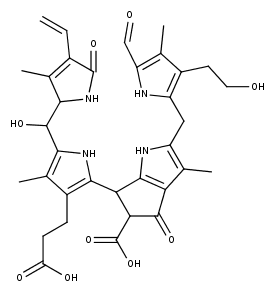
\includegraphics[width=\textwidth]{figures/Kapitel7/Kataboliten/fragmentation_structures/VWA_Katabolit_647.png}
    \caption{}
    \label{fig:NCC2725}
  \end{subfigure}
  \hfill
  \begin{subfigure}[b]{0.5\textwidth}
    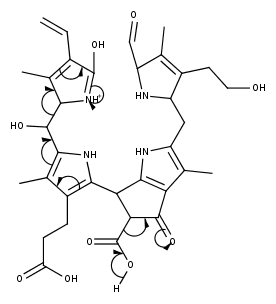
\includegraphics[width=\textwidth]{figures/Kapitel7/Kataboliten/fragmentation_structures/VWA_Katabolit_647-CO2-RingD_480_MH_electronMovement.png}
    \caption{}
    \label{fig:DNCC2991}
  \end{subfigure}
  \caption[Online-UV/Vis Spektren mit der Charakteristik eines NCC bei 27.10min., eines DNCC bei 29.75min. sowie eines YCC bei 30.94min., Quelle: Autor]{Online-UV/Vis Spektren: (a) charakteristisch für einen \gls{NCC} - RT = 27.25min., (b) charakteristisch für einen \gls{DNCC} - RT = 29.91min., (c) charakteristisch für einen \gls{YCC} - RT = 30.94min.}
\end{figure}

\begin{figure}[!htbp]
  \begin{subfigure}[b]{0.5\textwidth}
    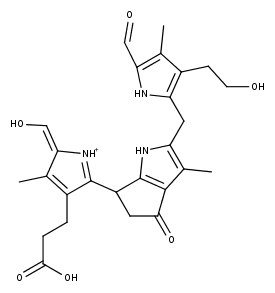
\includegraphics[width=\textwidth]{figures/Kapitel7/Kataboliten/fragmentation_structures/VWA_Katabolit_647-CO2-RingD_480_MH_Enolform.png}
    \caption{}
    \label{fig:NCC2725}
  \end{subfigure}
  \hfill
  \begin{subfigure}[b]{0.5\textwidth}
    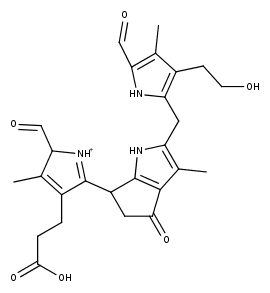
\includegraphics[width=\textwidth]{figures/Kapitel7/Kataboliten/fragmentation_structures/VWA_Katabolit_647-CO2-RingD_480_MH_Ketoform.png}
    \caption{}
    \label{fig:DNCC2991}
  \end{subfigure}
  \caption[Online-UV/Vis Spektren mit der Charakteristik eines NCC bei 27.10min., eines DNCC bei 29.75min. sowie eines YCC bei 30.94min., Quelle: Autor]{Online-UV/Vis Spektren: (a) charakteristisch für einen \gls{NCC} - RT = 27.25min., (b) charakteristisch für einen \gls{DNCC} - RT = 29.91min., (c) charakteristisch für einen \gls{YCC} - RT = 30.94min.}
\end{figure}

\subsection{Bo-NCC-1}

\begin{figure}[!htbp]
  \centering
  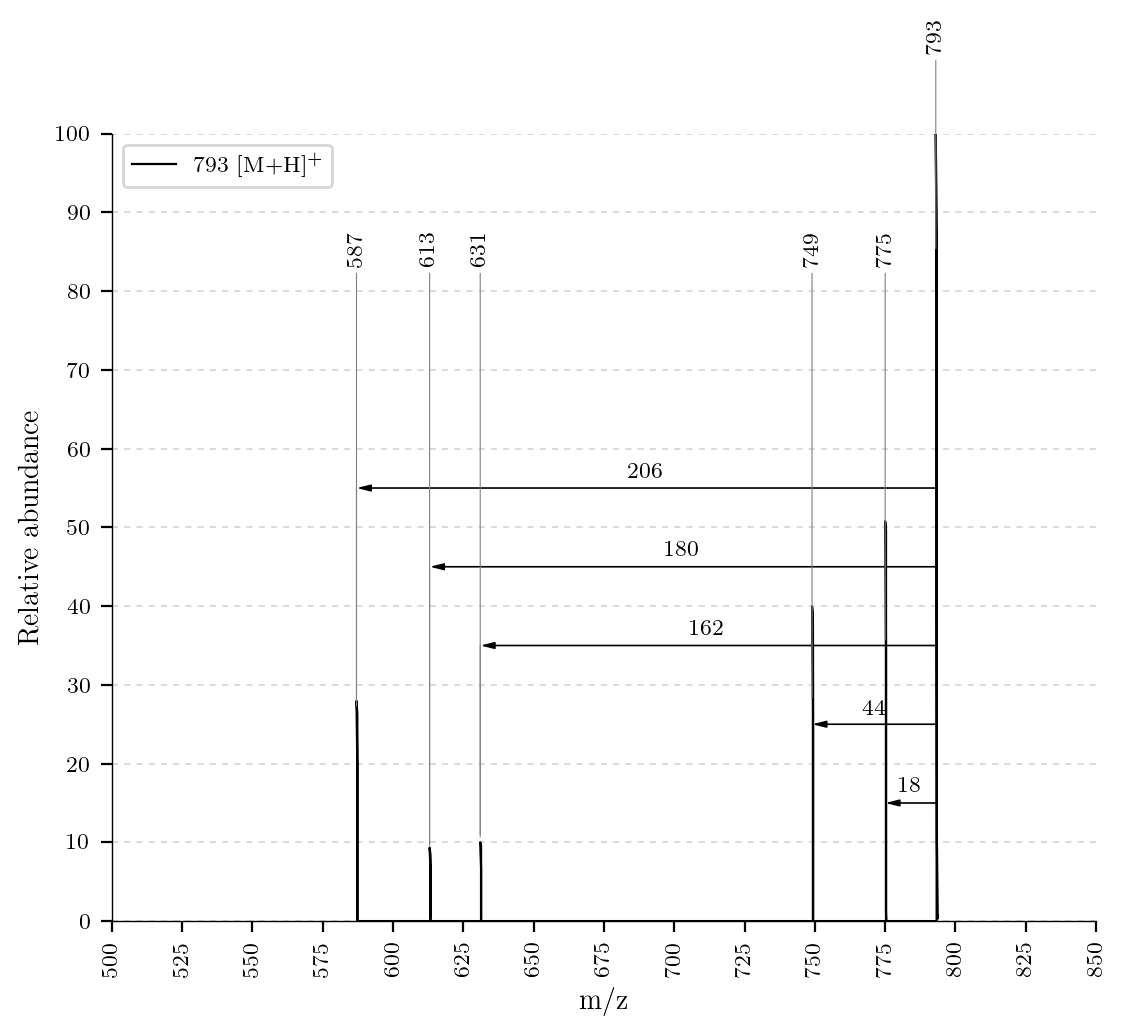
\includegraphics[width=\textwidth, height=0.7\textwidth]{figures/Kapitel7/Kataboliten/VWA_MS_793.png}
  \caption[LC-MS Chromatogramm vor der Reaktion, Quelle: Author]{\gls{lcms} Chromatogramm}
  \label{fig:LCMSChromatogramm}
\end{figure}



\section{Reaktionsprodukte der Chl-Kataboliten}

\subsection{Reaktionsprodukt von Bo-DYCC}

\begin{figure}[!htbp]
  \centering
  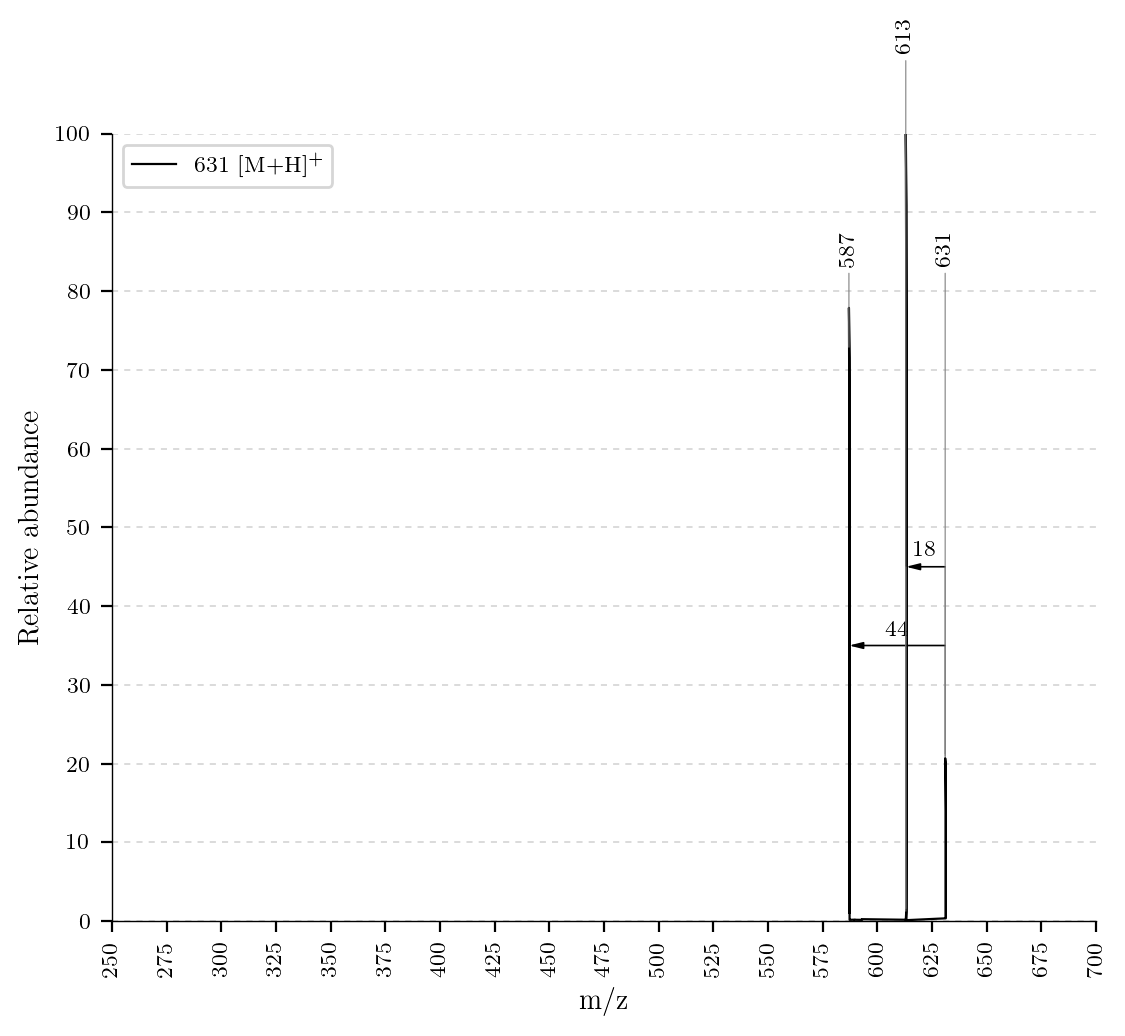
\includegraphics[width=\textwidth, height=0.7\textwidth]{figures/Kapitel7/Kataboliten/VWA_MS_631.png}
  \caption[LC-MS Chromatogramm vor der Reaktion, Quelle: Author]{\gls{lcms} Chromatogramm}
  \label{fig:LCMSChromatogramm}
\end{figure}

\begin{figure}[!htbp]
  \centering
  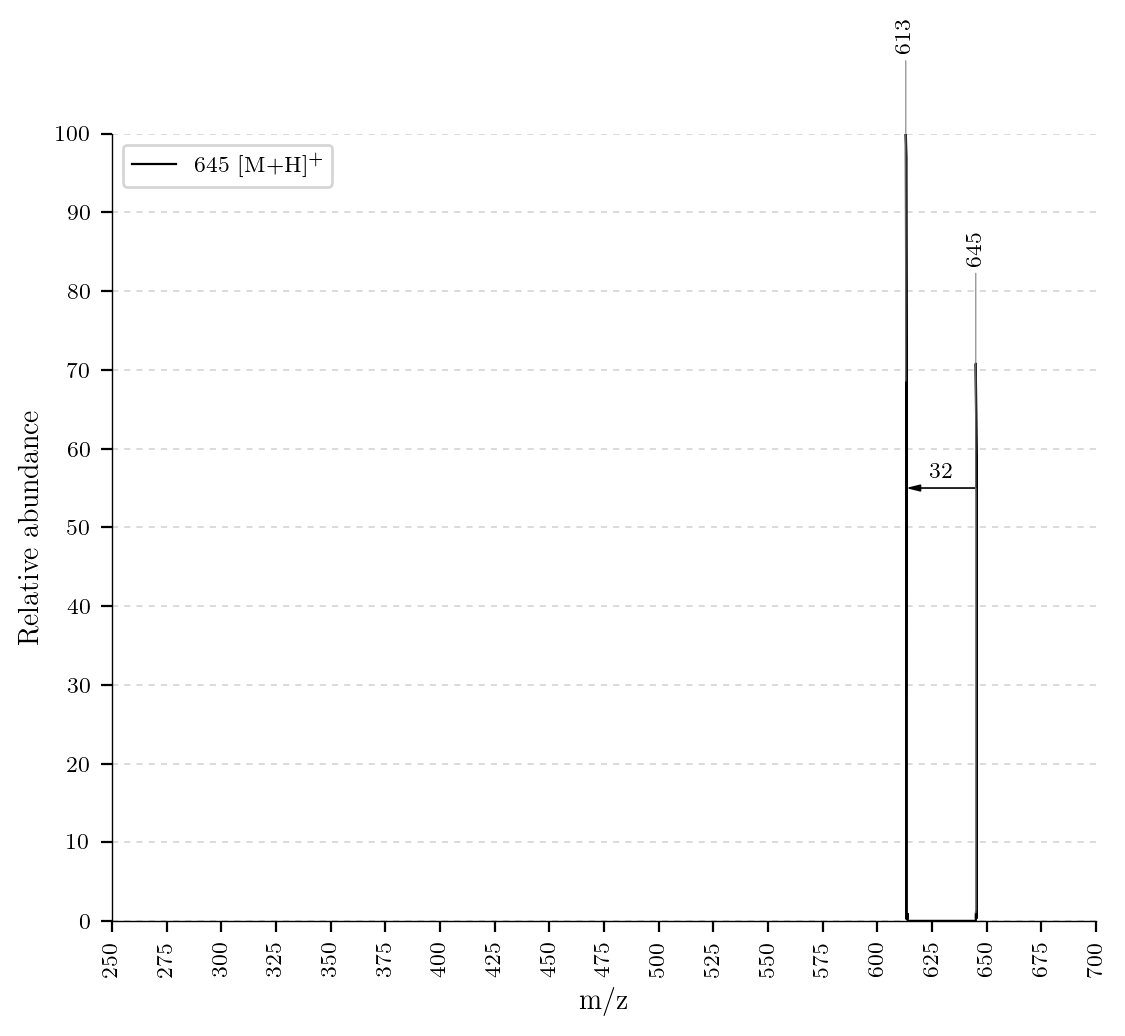
\includegraphics[width=\textwidth, height=0.7\textwidth]{figures/Kapitel7/Kataboliten/VWA_MS_645-2.png}
  \caption[LC-MS Chromatogramm vor der Reaktion, Quelle: Author]{\gls{lcms} Chromatogramm}
  \label{fig:LCMSChromatogramm}
\end{figure}


\begin{figure}[!htbp]
  \begin{subfigure}[b]{0.5\textwidth}
    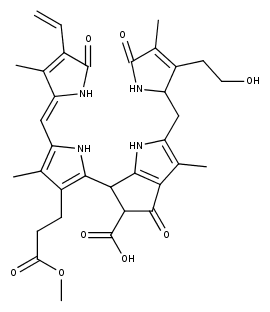
\includegraphics[width=\textwidth]{figures/Kapitel7/Kataboliten/fragmentation_structures/VWA_Katabolit_631.png}
    \caption{}
    \label{fig:NCC2725}
  \end{subfigure}
  \hfill
  \begin{subfigure}[b]{0.5\textwidth}
    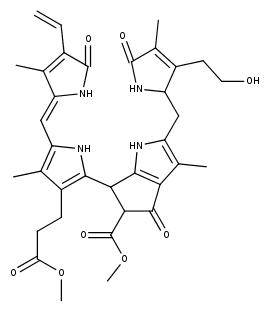
\includegraphics[width=\textwidth]{figures/Kapitel7/Kataboliten/fragmentation_structures/VWA_Katabolit_645_nachReaktion.png}
    \caption{}
    \label{fig:DNCC2991}
  \end{subfigure}
  \caption[Online-UV/Vis Spektren mit der Charakteristik eines NCC bei 27.10min., eines DNCC bei 29.75min. sowie eines YCC bei 30.94min., Quelle: Autor]{Online-UV/Vis Spektren: (a) charakteristisch für einen \gls{NCC} - RT = 27.25min., (b) charakteristisch für einen \gls{DNCC} - RT = 29.91min., (c) charakteristisch für einen \gls{YCC} - RT = 30.94min.}
\end{figure}

\subsection{Reaktionsprodukt von Bo-DNCC}

\begin{figure}[!htbp]
  \centering
  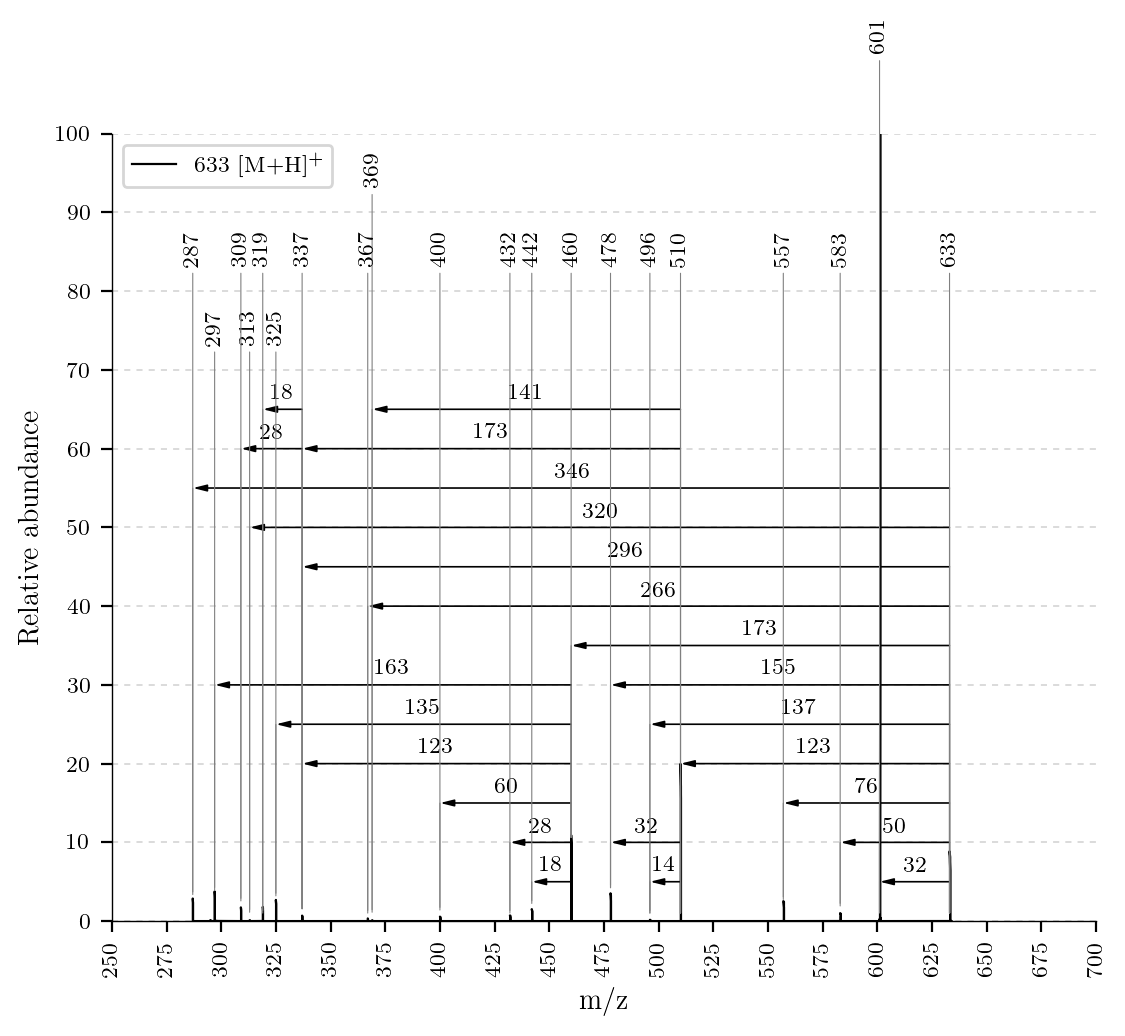
\includegraphics[width=\textwidth, height=0.7\textwidth]{figures/Kapitel7/Kataboliten/VWA_MS_633.png}
  \caption[LC-MS Chromatogramm vor der Reaktion, Quelle: Author]{\gls{lcms} Chromatogramm}
  \label{fig:LCMSChromatogramm}
\end{figure}

\begin{figure}[!htbp]
  \centering
  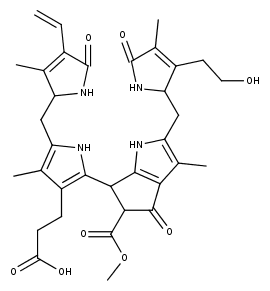
\includegraphics[scale=0.6]{figures/Kapitel7/Kataboliten/fragmentation_structures/VWA_Katabolit_633.png}
  \caption[LC-MS Chromatogramm vor der Reaktion, Quelle: Author]{\gls{lcms} Chromatogramm}
  \label{fig:LCMSChromatogramm}
\end{figure}

\subsection{Reaktionsprodukt von Bo-YCC}

Wurde nicht gefunden.

\subsection{Reaktionsprodukt von Bo-NCC-3}

\begin{figure}[!htbp]
  \centering
  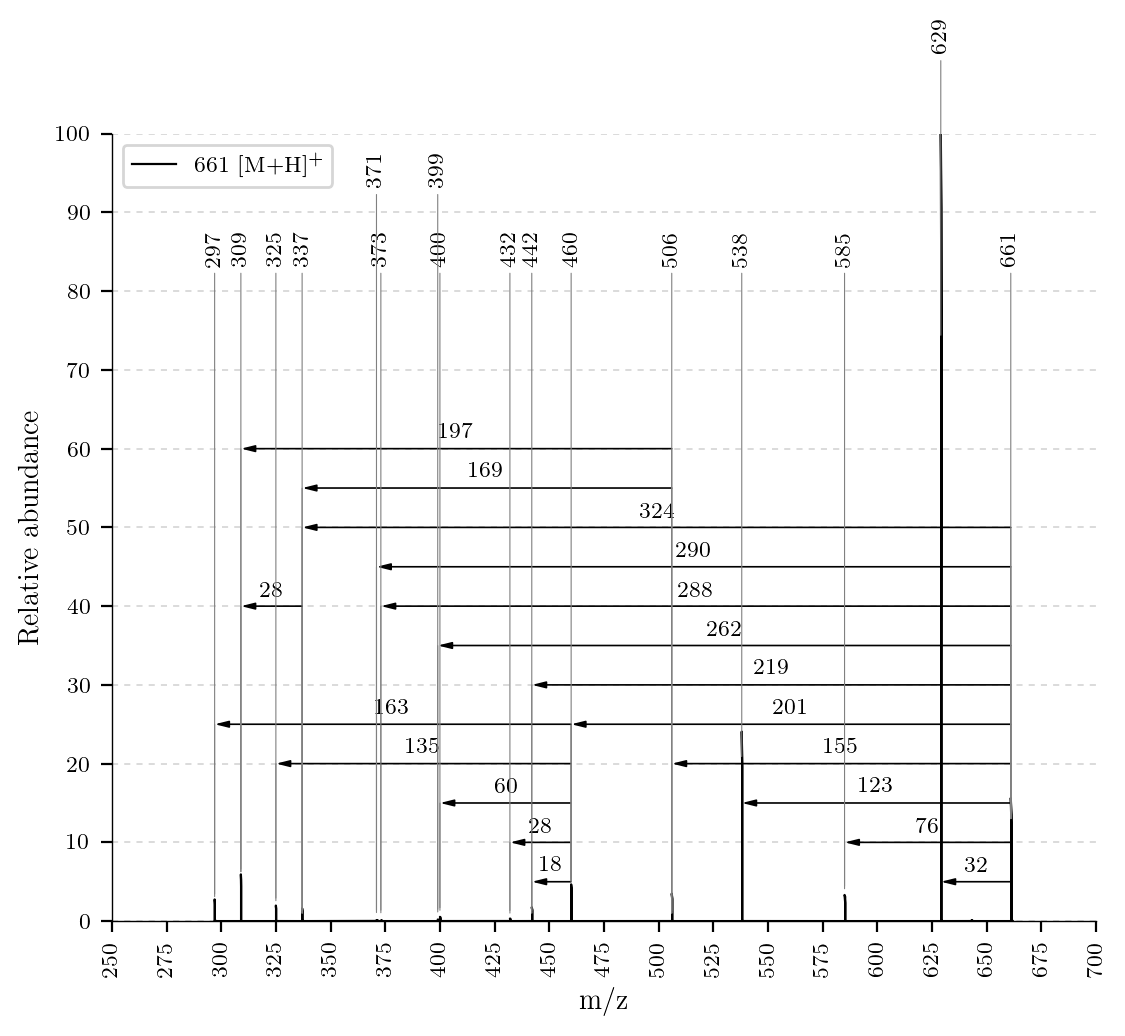
\includegraphics[width=\textwidth, height=0.7\textwidth]{figures/Kapitel7/Kataboliten/VWA_MS_661.png}
  \caption[LC-MS Chromatogramm vor der Reaktion, Quelle: Author]{\gls{lcms} Chromatogramm}
  \label{fig:LCMSChromatogramm}
\end{figure}

\subsection{Reaktionsprodukt von Bo-NCC-1}

Wurde nicht gefunden.
